%------------PREAMBLE
\include{preamble}
\usepackage{morefloats}
%---------------------------
                                          
%---------------------------

%---------------------------TABLE OF CONTENTS

%---------------------------

%---------------------------MAIN BODY
\documentclass{article}
\usepackage{graphicx} % Required for inserting images

\title{BTW Sandpile Model Report}
\author{Ruth Roberts }
\date{The Art of Scientific Communication}
\usepackage[dvipsnames, svgnames]{xcolor}
\usepackage{tikz}
\usetikzlibrary{shapes.geometric, arrows.meta, positioning}
\usepackage{amsmath}
\usepackage{amsthm}
\usepackage{amssymb}
\usepackage[utf8]{inputenc}
\usepackage[T1]{fontenc}
\usepackage{mathtools}
\usepackage{pgfplots}
\usepackage{float} 
\pgfplotsset{compat=1.18} % Recommended to set a compatibility level
\DeclareMathOperator{\E}{\mathbb{E}}
\DeclareMathOperator{\V}{\text{Var}}
\DeclareMathOperator{\C}{\text{Cov}}
\begin{document}
\maketitle
\tableofcontents

\section{Introduction: The Sandpile Model }
\subsection{Self Organised Criticality and Scale Invariance}
The Sandpile model was first introduced by Bak, Tang and Wiesenfeld as a basic example of what they called self organised criticality, a property of systems with large degrees of freedom characterised by scale invariance, meaning the "shape" of the system is the same regardless of the length scale chosen. The Bak, Tang and Wiesenfeld (BTW) Sandpile model was introduced in order to explain $\frac{1}{f}$ noise present in many physical phenomena, from resistors to stars. In mathematics, if a function is described as scale invariance this means that the function looks essentially the same whether the scale is small or large. These functions are typically characterised by power laws. This is demonstrated by the following plots of $f(x) = 2x^3$, on different scales: 

\begin{center}
    
\begin{tikzpicture}
  \begin{axis}[
      axis lines=center, % Places the axes in the middle
      xlabel={$x$},
      ylabel={$f(x)$},
      domain=-10:10,       % Sets the x-range
      samples=100        % More samples make the curve smoother
  ]
    \addplot[BrickRed, thick] {2*x^3}; 
  \end{axis}
\end{tikzpicture}
\end{center}
\begin{center}
\begin{tikzpicture}
  \begin{axis}[
      axis lines=center, % Places the axes in the middle
      xlabel={$x$},
      ylabel={$f(x)$},
      domain=-50:50,       % Sets the x-range
      samples=200        % More samples make the curve smoother
  ]
    \addplot[BrickRed, thick] {2*x^3}; 
  \end{axis}
\end{tikzpicture}
\end{center}

Power laws are a sign of scale invariance because they are dependent only on some multiplication of the input value with itself and a constant of proportionality:
\[f(x) = ax^b.\]
As a result, when we "zoom out" in the function, as we do in changing the scale from $[-10, 10]$  to $[-100,100]$ in the plots above. We have effectively multiplied the $x$ values by 10 and in doing so, multiplied the y values by $10^3$, only changing the constant of proportionality. 

\begin{center}
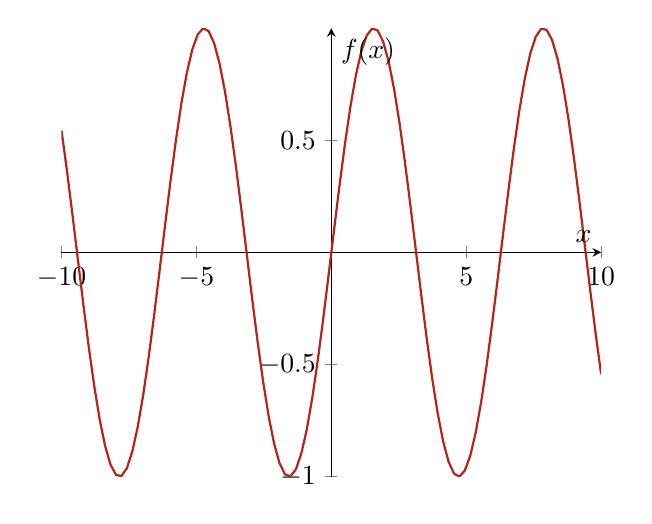
\begin{tikzpicture}
  \begin{axis}[
      axis lines=center, % Places the axes in the middle
      xlabel={$x$},
      ylabel={$f(x)$},
      domain=-10:10,       % Sets the x-range
      samples=100        % More samples make the curve smoother
  ]
    \addplot[BrickRed, thick] {sin(deg(x))}; 
  \end{axis}
\end{tikzpicture}
\end{center}

\begin{center}
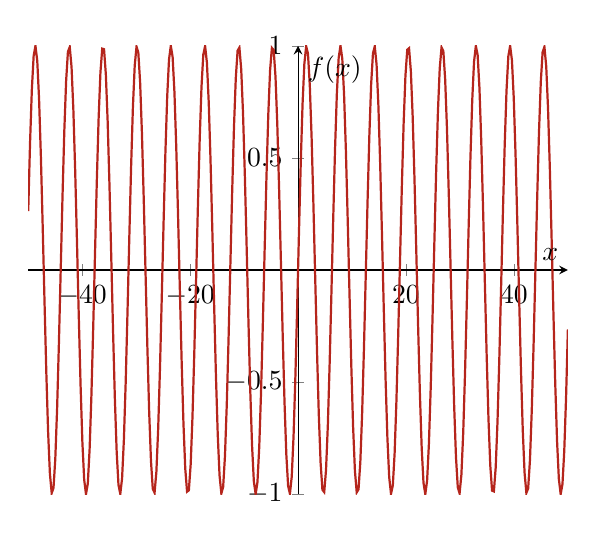
\begin{tikzpicture}
  \begin{axis}[
      axis lines=center, % Places the axes in the middle
      xlabel={$x$},
      ylabel={$f(x)$},
      domain=-50:50,  
      samples=300        % More samples make the curve smoother
  ]
    \addplot[BrickRed, thick] {sin(deg(x))}; 
  \end{axis}
\end{tikzpicture}
\end{center}

We see that there are many more periods when plotted over more values of $x$, so the two plots do not have the same shape as the plots of $f(x) = 2x^3$ id. 

\subsection{The Sandpile Model}
The sandpile model models piles of grains of sand on a square two-dimensional lattice. A grain of sand is added to a site chosen uniformly at random each timestep, and there is some threshold value (usually taken to be 4 on a two-dimensional lattice) at which a pile becomes unstable and "topples", distributing its grains of sand to neighbouring piles. This can cause the neighbouring piles to topple, causing an "avalanche" which, with large grids, can consist of hundreds or even thousands of topples. For example, consider the following stable $3 \times 3$ lattice, where darker green corresponds to more grains of sand in the pile (ranging from 0 to 3 grains):
\begin{center}

\begin{tikzpicture}
  % each square: \fill[color] (x,y) rectangle (x+1,y+1);
  \fill[YellowGreen!60!OliveGreen]  (0,0) rectangle (1,1);
  \fill[OliveGreen] (1,0) rectangle (2,1);
  \fill[YellowGreen!60!OliveGreen] (2,0) rectangle (3,1);
  \fill[OliveGreen]   (0,1) rectangle (1,2);
  \fill[OliveGreen](1,1) rectangle (2,2);
  \fill[YellowGreen]  (2,1) rectangle (3,2);
  \fill[YellowGreen](0,2) rectangle (1,3);
  \fill[YellowGreen!60!OliveGreen]   (1,2) rectangle (2,3);
  \fill[YellowGreen!2!OliveGreen](2,2) rectangle (3,3);
\end{tikzpicture}
\end{center}
Now imagine a grain of sand is dropped on the centre of the lattice, taking it above the threshold (represented by the red square):
\begin{center}

\begin{tikzpicture}
  % each square: \fill[color] (x,y) rectangle (x+1,y+1);
  \fill[YellowGreen!60!OliveGreen]  (0,0) rectangle (1,1);
  \fill[OliveGreen] (1,0) rectangle (2,1);
  \fill[YellowGreen!60!OliveGreen] (2,0) rectangle (3,1);
  \fill[OliveGreen]   (0,1) rectangle (1,2);
  \fill[BrickRed](1,1) rectangle (2,2);
  \fill[YellowGreen]  (2,1) rectangle (3,2);
  \fill[YellowGreen](0,2) rectangle (1,3);
  \fill[YellowGreen!60!OliveGreen]   (1,2) rectangle (2,3);
  \fill[YellowGreen!2!OliveGreen](2,2) rectangle (3,3);
\end{tikzpicture}
\end{center}

The pile then topples and redistributes grains to its neighbours:
\begin{center}

\begin{tikzpicture}
  % each square: \fill[color] (x,y) rectangle (x+1,y+1);
  \fill[YellowGreen!60!OliveGreen]  (0,0) rectangle (1,1);
  \fill[BrickRed] (1,0) rectangle (2,1);
  \fill[YellowGreen!60!OliveGreen] (2,0) rectangle (3,1);
  \fill[BrickRed]   (0,1) rectangle (1,2);
  \fill[YellowGreen](1,1) rectangle (2,2);
  \fill[YellowGreen!60!OliveGreen]  (2,1) rectangle (3,2);
  \fill[YellowGreen](0,2) rectangle (1,3);
  \fill[YellowGreen!2!OliveGreen]   (1,2) rectangle (2,3);
  \fill[YellowGreen!2!OliveGreen](2,2) rectangle (3,3);
\end{tikzpicture}
\end{center}
Now we see that two more piles need toppling. Because of the Abelian property of the Sandpile Model, (which will be discussed in more detail later) regardless of which site we topple first, the final configuration of the lattice will be the same. We continue toppling until the lattice is stable, meaning all values are below the threshold. 
\begin{center}

\begin{tikzpicture}
  % each square: \fill[color] (x,y) rectangle (x+1,y+1);
  \fill[YellowGreen!2!OliveGreen]  (0,0) rectangle (1,1);
  \fill[YellowGreen] (1,0) rectangle (2,1);
  \fill[YellowGreen!2!OliveGreen] (2,0) rectangle (3,1);
  \fill[BrickRed]   (0,1) rectangle (1,2);
  \fill[YellowGreen!60!OliveGreen](1,1) rectangle (2,2);
  \fill[YellowGreen!60!OliveGreen]  (2,1) rectangle (3,2);
  \fill[YellowGreen](0,2) rectangle (1,3);
  \fill[YellowGreen!2!OliveGreen]   (1,2) rectangle (2,3);
  \fill[YellowGreen!2!OliveGreen](2,2) rectangle (3,3);
\end{tikzpicture}
\end{center}

\begin{center}

\begin{tikzpicture}
  % each square: \fill[color] (x,y) rectangle (x+1,y+1);
  \fill[OliveGreen]  (0,0) rectangle (1,1);
  \fill[YellowGreen] (1,0) rectangle (2,1);
  \fill[YellowGreen!2!OliveGreen] (2,0) rectangle (3,1);
  \fill[YellowGreen]   (0,1) rectangle (1,2);
  \fill[YellowGreen!2!OliveGreen](1,1) rectangle (2,2);
  \fill[YellowGreen!60!OliveGreen]  (2,1) rectangle (3,2);
  \fill[YellowGreen!60!OliveGreen](0,2) rectangle (1,3);
  \fill[YellowGreen!2!OliveGreen]   (1,2) rectangle (2,3);
  \fill[YellowGreen!2!OliveGreen](2,2) rectangle (3,3);
\end{tikzpicture}
\end{center}
This is a simple illustrative example, but it is easy to see how the dynamics of this model can get quite complicated on a large lattice as there are many degrees of freedom due to the amount of individual piles of sand. This is where the self organised criticality of the system comes from.

\subsection{The Abelian Property}

The Abelian property is fundamental to understanding and simulating BTW Sandpile models. Informally, an operation has the Abelian property if, when applied multiple times, the order of the operations does not change the end result. That is, the order with which we apply the operations does not affect the end result. For example, the basic operations addition and multiplication on the set of real numbers have the Abelian property while subtraction and division do not. To show how the toppling operator in the BTW model satisfies this property, I will define the toppling operator mathematically and explain how the order of topples does not impact the end result.
\newline
Consider an $n\times n$ lattice $L$ and a site on the lattice $(i, j)$. We represent the lattice as a matrix with $l^{(ij)}$ denoting the number of grains of sand in the pile at site $(i, j)$. Let $T_{ij}$ be the toppling operator for site $(i,j)$. Then we can define a matrix $\Delta_{ij}$ such that $T_{ij}(L, (i,j)) = L + \Delta_{ij}$. Then, for a $d$ dimensional lattice, we have:
\[
\delta_{ij}^{(i'j')} = \left\{
\begin{array}{ll}
      -4, & \text{if } i'=i, j'=j \\
      1, & \text{if } i'=i\pm1 \text{ and/or } j'=j\pm1\\ 
      0, & \text{otherwise.}
\end{array} 
\right.
\]
Hence, if we take multiple sites $(i_1,j_1), (i_2, j_2), (i_3, j_3)$ in a lattice $L$, toppling these sites is the same as adding $\Delta_{i_1j_1}, \Delta_{i_2j_2} \text{ and } \Delta_{i_3j_3}$ to the lattice $L$, which is essentially addition in $\mathbb{R}^n$ so is commutative. Hence, the model is Abelian as long as the order of toppling sites does not affect the sites that will be toppled. This is clearly the case because the only way for an unstable site to become stable again is by being toppled, meaning once a site becomes unstable, it can only become "more" unstable (receive grains of sand from toppled neighbours) in which case it will still topple.
\subsection{Simulating the BTW Model}
In this project I will simulate a BTW model on a various square lattices (side lengths 80, 90, 100, 110 and 120)over 500000 timesteps, recording and analysing the following statistics for each avalanche:
\newline
\newline
\textbf{Area}: the number of sites toppled in the avalanche.
\newline
\newline
\textbf{Length} (radius): The Manhattan distance between the first site toppled (the site which received the dropped sand) and the furthest site whose pile size has been affected in the avalanche. This could be a site that is toppled or the neighbour of a site that has been toppled meaning the pile at the site has increased in size without needing to be toppled.
\newline
\newline
\textbf{Topples}: The number of topples occurring in the avalanche.
\newline
\newline
\textbf{Loss}: The number of grains of sand lost at the boundary of the lattice during the avalanche. 
\newline
\newline
\textbf{Mass}: The number of grains of sand in the whole grid
\newline
 \subsection{Predictions}
Because grains of sand are added to the model at random and can be lost , I do not expect the system to reach a steady state, where properties of avalanches or statistics of the lattice itself are constant over time. For the same reason, I do not expect the number of grains of sand in the lattice to reach an equilibrium state. However, I would expect the system to reach a statistically stationary state, where the statistical distributions of properties of avalanches and the lattice itself do not change over time. I would also expect the average number of grains of sand in the lattice and grains of sand in each site to remain constant; once there are enough grains of sand (two or three grains at most sites in the interior of the lattice), any site in the interior that is toppled is fairly likely to have its pile replenished by the avalanches of its neighbours. This was the case in the example above, where the central site finished the avalanche with two grains of sand in its pile due to the avalanches of two of its neighbours. This average cannot be too close to three, because the large avalanches would cause many grains to spill over the edge, significantly decreasing the average size of piles across the lattice. It also cannot be too small; there must be a significant proportion of the piles which have size three, otherwise avalanches and topples will be very infrequent. Simulating the lattice must be done with finite boundaries because the computer cannot store and operate on an infinite array. Furthermore, the number of different possible configurations of pile sizes on an infinite lattice would not be countable.
\newpage
\section{Methodology}
\subsection{Code Outline}
The basic structure of my code for simulating the sandpile model was to initialise a lattice of zeroes, then every timestep, drop a grain of sand on a randomly chosen site from the grid. I then called my avalanche function, which repeatedly called the topple function for unstable sites to redistribute grains of sand to their neighbours until the grid was stable again. A flow chart is included on the next page to show the structure of the code. 

\subsection{The Topple and Avalanche Functions}
The actual simulation of the lattice using the Topple and Avalanche functions were actually quite simple. Once the sand has been dropped, the avalanche function checks for unstable sites. If a site is found, it is added to a global set called "affected sites". While affected sites is non empty, a site is chosen from the set and, if the pile of sand at the site is at or above the threshold, the topple function is called for the site, meaning the pile at that site loses four of its grains of sand and each of its neighbours gains a grain of sand. Within the toppling function, these neighbours are also added to the set "affected sites". I had initially done this in the avalanche function, but this meant that I had to check neighbours twice for each topple, once in the topple function to check if a grain should be added, and once in the avalanche function to check if the neighbour should be added to affected sites. Doing this in the toppling function sped up my code by a few seconds. The neighbours may not be at or above the threshold, which is why each site from "affected sites" is checked before it is toppled. The set is used to avoid having to check the whole grid for unstable sites after each topple, of which there can be thousands per timestep. This is enough to simulate the lattice, in fact, there are faster methods of doing so using vectorisation and performing multiple topples at once. However, such methods make it difficult to keep track of the relevant statistics for each avalanche.
\begin{center}
\tikzstyle{box} = [rectangle, rounded corners, minimum width=3cm, minimum height=1cm, text centered, draw=black, fill=ForestGreen!60]
\tikzstyle{decision} = [diamond, aspect=2, minimum width=3cm, minimum height=1cm, text centered, draw=black, fill=YellowGreen!60]
\tikzstyle{arrow} = [thick, ->, >=stealth]

\begin{tikzpicture}[node distance=2cm]

  \node (drop)      [box]                          {Drop Sand};
  \node (avalanche) [box, below of=drop]      {Avalanche?};
  \node (stable1)   [decision, below of=avalanche] {Stable?};
  \node (topple)    [box, below of=stable1]        {Topple};
  \node (stable2)   [decision, below of=topple]    {Stable?};
  \node (burnin)    [decision, below of=stable2]   {Burn-in complete?};
  \node (update)    [box, below of=burnin]         {Update Statistics};
  \node (done)      [box, below of=update]         {New Timestep};

  % main flow
  \draw [arrow] (drop)      -- (avalanche);
  \draw [arrow] (avalanche) -- (stable1);
  \draw [arrow] (stable1)   -- node[anchor=east] {No}  (topple);
  \draw [arrow] (topple)    -- (stable2);

  % stable2 No loops back to topple
  \draw [arrow] (stable2.east) -- ++(1.5,0) node[anchor=west] {No} 
      |- (topple.east);

  % stable1 Yes skips to burnin
  \draw [arrow] (stable1.west) -- ++(-1.5,0) node[anchor=east] {Yes} 
      |- (done.west);

  % stable2 Yes goes to burnin
  \draw [arrow] (stable2) -- node[anchor=east] {Yes} (burnin);


  % burnin
  \draw [arrow] (burnin)  -- node[anchor=east] {Yes} (update);
  \draw [arrow] (update)  -- (done);

  % burnin No goes to done
  \draw [arrow] (burnin.east) -- ++(3.5,0) node[anchor=west] {No} 
      |- (done.east);
  \draw [arrow] (done.south) -- ++(0,-0.75) 
      -- ++(-5,0) 
      |- (drop.west);
\end{tikzpicture}
\end{center}
\subsection{Recording Statistics}
I recorded all of the statistics at the end of each timestep in the "[statistic]\_history" array, and used default dictionaries "[statistic]\_counts" to count the number of times each statistic recorded a certain value. I found the statistics using "curr\_[statistic]" which was either updated progressively during the avalanche or topples, or was updated at the end of the avalanche.
\newline
\textbf{Mass}: curr\_mass is incremented in the drop\_sand function, then decreased by four in the topple function every time a topple occurs before being increased by one for each neighbour that is inside the grid.
\newline
\newline
\textbf{Area}: at the start of each avalanche a local set, "toppled\_sites" is initialised to contain any sites that are unstable (which can only be one or zero initially). Before a site  is toppled, it is added to toppled\_sites within the avalanche function. At the end of the avalanche, curr\_area is set to be the length of toppled\_sites. 
\newline
\newline
\textbf{Topples}: curr\_topples is increased by one every time the avalanche function calls the topple function
\newline
\newline
\textbf{Loss}: at the end of the avalanche, curr\_loss is defined as follows: 

\[\text{curr\_loss} = \text{mass\_history[curr
\_time-1]} - \text{curr\_mass} + 1,\] with the extra $1$ accounting for the fact that a grain of sand has been added during the timestep, and with mass\_history[curr
\_time-1] being the mass of the grid at the previous timestep. 
\newline
\newline
\textbf{Length}: length was the most complicated to calculate. For each site in toppled\_sites, the Manhattan distance to the initial\_site is calculated. If the site is not a corner of the lattice, the distance associated with this site is set to be one more than the Manhattan distance, since at least one of the neighbours of this site will have a Manhattan distance from initial\_site that is further. If the site is a corner of the lattice, this is not the case, so the distance associated with this site set to be the Manhattan distance from this site to initial\_site. I appended each of these distances to a list, "lengths" and then set curr\_length to be the maximum value in lengths. To determine whether sites were corners, I initialised a list of corner sites in the \_\_init\_\_ function for the class and checked whether the site is in that list. 
\newline
\newline
\textbf{Time Average}: I initialised a grid of zeroes, then in the run() function, after each timestep I added the current grid to space average history, then at the end divided by the number of at the end to get the average pile size at each site over time.
\newline
\newline
\textbf{Space Average History}: I initialised an array of zeroes with the same length as the number of timesteps, then set space\_average\_history[curr\_]  time  to be the mass of the grid divided by the number of sites in the grid. 

\subsection{Burn-In}
I defined the functions "find\_stats" and "update\_stats" to find the statistics at the end of each avalanche and add them to the counts dictionaries only once the burn-in period was finished, ($\textbf{curr\_time}>\textbf{burn\_in}$) so that I did not have to use time calculating statistics that I did not need. To determine what the burn-in should be, I ran my code to make lattices for square grids with side lengths 20, 40, 60, 80 and 100 and plotted the space\_average\_history over time for each of them to determine roughly where it begins to plateau. These lattices were overfall smaller than the ones I would evenutally analyse because I wanted to find an estimate for the burn-in period before running the code on large lattices to save time. As seen from these plots, the point where it begins to plateau was quite easy to see by inspection. I then plotted the timesteps needed to plateau vs the area of the grid, which was linear as shown below and found the linear regression formula (with y intercept set to 0) to find the constant of proportionality. I then set burn\_in to be this constant times the number of sites in the lattice. This may not work as well for rectangular lattices, which can be simulated using my code, but my analysis focuses on square lattices anyway. 

\begin{figure}[H]
    \centering
    \includegraphics[width=0.5\linewidth]{20by20.png}
    \caption{Space Average over Time for 20x20 Lattice}
    \label{fig:20}
\end{figure}

\begin{figure}[H]
    \centering
    \includegraphics[width=0.5\linewidth]{40by40.png}
    \caption{Space Average over Time for 40x40 Lattice}
    \label{fig:40}
\end{figure}

\begin{figure}
    \centering
    \includegraphics[width=0.5\linewidth]{60by60.png}
    \caption{Space Average over Time for 60x60 Lattice}
    \label{fig:60}
\end{figure}

\begin{figure}
    \centering
    \includegraphics[width=0.5\linewidth]{80by80.png}
    \caption{Space Average over Time for 80x80 Lattice}
    \label{fig:80}
\end{figure}

\begin{figure}
    \centering
    \includegraphics[width=0.5\linewidth]{100by100.png}
    \caption{Space Average over Time for 100x100 Lattice}
    \label{fig:100}
\end{figure}

\begin{figure}
    \centering
    \includegraphics[width=0.5\linewidth]{burnin.png}
    \caption{Burn In}
    \label{fig:burnin}
\end{figure}

\section{Results}
\subsection{Ergodicity}
Because the system reaches a statistically stationary state after the burn-in period, the system is also ergodic, meaning if we were to take 10,000 such systems which had already reached a statistically stationary state and sample a single avalanche from each, we would get the same distributions for each statistic as if we were to sample one such system 10,000 times. This only applies once the system has reached the statistically stationary state because ergodicity in these systems, which can be thought of as a Discrete Time Markov Chain with a very large (but finite when the lattice is finite) number of states due to the fact that the configuration in one timestep solely determines the likelihood of each potential configuration in the next timestep. In this system, configurations with a smaller average pile size across the grid (roughly less than 2) are not recurrent; once the system reaches these configurations it will likely not return. Instead, the system moves between configurations around this statistically stationary state, which mostly includes configurations with average pile size just over 2, depending on the size of the lattice. There is only one recurrent state, so within this state, the Markov Chain is irreducible and aperiodic and therefore ergodic. 

\subsection{Fitting the Power Law}
To test whether the different statistics follow the power laws expected for self organised criticality I used the counts dictionaries to plot log-log plots of the the number of occurrences of a particular value of a statistic (after the burn-in period) vs the value of the statistic. Using the log-log plots, it was evident that area, length and topples all followed power law, while loss did not as the log-log plot did not look linear.
\newline
I investigated how the power law changed for different sized lattices using square lattices with side lengths 80, 90, 100, 110 and 120. The tables below show the power laws that I obtained for each statistic and size of lattice. Calculating this power law proved to be quite a challenging process as the plots, look less linear for the largest values of $\log(\text{statistic})$, since the number of occurrences of larger values of statistics tend to be close to zero and there are not enough occurrences of these for them to be likely to have converged to near their expected value. It was clear that I should discard some of these to enable the linear fit to better reflect those data points which I thought were more likely to be well estimated from the model. However, deciding how to discard these and how many was not simple. I wanted to keep my method consistent for each grid size, so I (with some help from AI) came up with three potential methods to discard values.
\newline
The simplest method was just to discard some proportion of the values at the end. I experimented with different proportions and how they affected the final plots. The advantage of discarding more values (even keeping only one tenth) was that these values represented more avalanches from my simulation and since the probability of smaller statistics was higher, I expected that these values would be better estimated in the model. However, were I to discard too many of the extreme values, I would lose key properties of the statistics themselves and the grid size. For example, the more extreme values I discarded, the closer my exponents for topples and area were, because it is particularly in the extreme values that the number of topples is much larger than the area of an avalanche. Additionally, the differences between grid sizes were being ignored as the avalanches with the largest amount of topples, for instance, were being ignored, but it is these avalanches which can show the distinction between, for instance, simulations on a 100 by 100 lattice and a 110 by 110 lattice. Eventually, I decided to keep one third of the values, discarding the last two thirds of the values, to maintain this balance. 
\newline
Another method I tried was using piecewise\_regression function in python. Since the drop off at the end itself looked fairly linear, I thought that piecewise\_regression might be able to split the plots into two parts, and I could take the linear regression law for the first part. However, for larger lattices, the plots were more consistently linear and piecewise\_regression failed to converge and split the plots into two parts, while for smaller lattices, the drop off point was not clear enough and piecewise\_regression often fit a line which included too many extreme values worsening the fit for the lower values which I believed were better estimated. 
\newline
The final method I tried was using ransac\_regressor to create a mask of values which it determined did not fit as well as the others, and then omit these values. This was sometimes quite effective, however, because the function tests points at random to discard, sometimes when the function chose too many points from extreme values of the particular statistic, the fits were way off. Additionally, it did not reflect the fact that I wanted to discard larger values for the statistics.
\newline
Due to the constraints of the latter two methods, along with their increased time needs, I decided to use the first, simpler method to find the fit for each statistic and lattice. 
The plots for the 100 by 100 lattice are displayed below. I also included the log-log plot for loss to demonstrate its non-linearity although I did not fit a linear regression to it.

\begin{figure}[H]
    \centering
    \includegraphics[width=0.5\linewidth]{loglogarea.png}
    \caption{Log-Log Plot for Area}
    \label{fig:lla}
\end{figure}

\begin{figure}[H]
    \centering
    \includegraphics[width=0.5\linewidth]{logloglength.png}
    \caption{Log-Log Plot for Length}
    \label{fig:lll}
\end{figure}

\begin{figure}[H]
    \centering
    \includegraphics[width=0.5\linewidth]{loglogtopples.png}
    \caption{Log-Log Plot for Topples}
    \label{fig:llt}
\end{figure}

The exponents I obtained for each statistic across the different sized lattices are displayed in the table below.
\begin{table}[H]
\centering
\begin{tabular}{|c|c|c|c|}
\hline
\textbf{Side Length} & \textbf{Area} & \textbf{Length} & \textbf{Topples}\\
\hline
80 & $-1.113$ & $-1.040$ & $-1.142$\\
90 & $-1.097$ & $-1.038$ & $-1.103$\\
100 & $-1.087$ & $-1.067$ & $-1.071$ \\
110 & $1.071$ & $-1.133$ & $-1.037$ \\
120 & $-1.056$ & $-1.109$ & $-1.008$ \\
\hline
\end{tabular}
\caption{Exponents for the Distribution of Statistics across Varying Grid Sizes}
\label{tab:power_laws}
\end{table}

The exponents for area and topples decrease with increasing grid size, getting closer to 1. This matches the theoretical application of BTW models in explaining $\frac{1}{f}$ noise. However, the length exponents are less consistent, fluctuating in these examples. This is probably due to the fact that the maximum length is constrained to twice the grid side length, meaning it is difficult to fit a power law, because if length followed a strict power law, there would theoretically be a small number of occurrences of avalanches with lengths above the maximum length. I also a plotted scatter plot (shown below) for the exponents at different grid sizes, which revealed a linear relationship between the exponents and the side length, although it should be noted that the lattice sizes are relatively close together so this may well not be linear over a wider range of lattice sizes. 

\begin{figure}[H]
    \centering
    \includegraphics[width=0.5\linewidth]{exponents.png}
    \caption{Exponents for Different Sized Lattices}
    \label{fig:exps}
\end{figure}


Once the linearity was confirmed, I fit polynomial distributions to these plots to determine the exponent associated with each statistic and the coefficient of proportionality. The polynomial fits are shown on the histograms below, except for the histogram for loss which is included without a polynomial fit as it does not follow a power law *these are not the actual plots i'm using but i haven't fixed it yet*: 

\begin{figure}[H]
    \centering
    \includegraphics[width=0.8\linewidth]{areavsfreq.png}
    \caption{Histogram for Area showing Polynomial Fit}
    \label{fig:area}
\end{figure}

\begin{figure}[H]
    \centering
    \includegraphics[width=0.8\linewidth]{lengthvsfreq.png}
    \caption{Histogram for Length showing Polynomial Fit}
    \label{fig:length}
\end{figure}

\begin{figure}[H]
    \centering
    \includegraphics[width=0.8\linewidth]{lossvsfreq.png}
    \caption{Histogram for Loss}
    \label{fig:loss}
\end{figure}

\begin{figure}[H]
    \centering
    \includegraphics[width=0.8\linewidth]{topplesvsfreq.png}
    \caption{Histogram for Topples showing Polynomial Fit}
    \label{fig:topples}
\end{figure}


\subsection{Correlation}
I expected significant positive correlation between topples and area, since topples is at least as big as area (and in many cases the same) and more likely to be larger than area if area is large. I also expected positive correlation between topples and length and area and length, although maybe not as much. I did expect some positive correlation between the three statistics and loss, but I was unsure how strong the correlation would be, since the loss would also depend on the site that triggers the avalanche; if this initial site is close to the edge of the lattices, it would be more likely that loss will occur in the resulting avalanche. But in this case the area and number of topples from the avalanche would be constrained as the spread would be constrained in at least one direction.
\newline
After simulating the 100 by 100 grid, I plotted correlation plots for each pair of statistics to see how they related to one another. The plots, displayed below, show interesting relationships between the statistics. For the correlation between length and area I plotted the square root of the area against the length since the correlation plot for length and area appeared to show a quadratic relationship. 

\begin{figure}[H]
    \centering
    \includegraphics[width=0.5\linewidth]{corrlea.png}
    \caption{Correlation Plot for Length and Square Root Area}
    \label{fig:cla}
\end{figure}

This plot supports the belief that there is a quadratic relationship between the length and the area of the avalanche, although the fan shape indicates heteroskedasticity, with the variance away from this linear relationship dependent on the magnitude of the observations. This is probably because the length measurement is taken from the initial site, which is not necessarily centered, especially for large avalanches. If the initial site is not near the centre of the sites affected by the resulting avalanche, as might be the case if the avalanche propagates from a site near the edge of the lattice, the length will be large compared to the size of the avalanche as the length measurement will be closer to a diameter than a radius. The length is typically longer than the square root of the area, which makes sense since the Manhattan distance, not the Euclidean distance was used.

\begin{figure}[H]
    \centering
    \includegraphics[width=0.5\linewidth]{corrlelo.png}
    \caption{Correlation Plot for Loss and Length}
    \label{fig:clelo}
\end{figure}

The plot shows that while there is more scope for higher loss from avalanches with a greater length, there are also many avalanches with very few grains of sand lost across all lengths.

\begin{figure}[H]
    \centering
    \includegraphics[width=0.5\linewidth]{corrloa.png}
    \caption{Correlation Plot for Loss and Area}
    \label{fig:cloa}
\end{figure}

This plot is similar to the plot for loss and length, showing many avalanches with smaller loss across different areas of avalanche, although the correlation between the two is stronger than in the previous plot with most of the avalanches with the most loss also having a larger area. 

\begin{figure}[H]
    \centering
    \includegraphics[width=0.5\linewidth]{corrta.png}
    \caption{Correlation Plot for Topples and Area}
    \label{fig:cta}
\end{figure}

As predicted, there are many avalanches for which the topples and area are the same or close to the same, although for avalanches with the largest area the number of topples for the avalanche is much larger, even almost 8 times larger than the area of the avalanche. Of course, the more sites topples, the more likely sites are to topple multiple times as grains of sand are transferred between interior sites over the course of many topples.

\begin{figure}[H]
    \centering
    \includegraphics[width=0.5\linewidth]{corrtle.png}
    \caption{Correlation Plot for Topples and Length}
    \label{fig:cte}
\end{figure}

The mountain shape of the correlation plot for topples and length reflects the fact that avalanches beginning near the centre are more likely to involve more topples, since grains can transfer between sites over many topples before the propagations reach the edge of the lattice and grains are lost. Avalanches with lengths between 150 and 200 have to start closer to the edges of the lattice for this length measurement to be possible, meaning the number of topples is limited by the 

\begin{figure}[H]
    \centering
    \includegraphics[width=0.5\linewidth]{corrtlo.png}
    \caption{Correlation Plot for Topples and Loss}
    \label{fig:ctlo}
\end{figure}

This plot seems to be the most linear, with even the variance apparently consistent and unaffected by the magnitude of the topples and/or loss. This suggests that whenever there are a lot of topples, these propagate to the edges of the lattice and cause significant loss of grains of sand over the edge, with this loss linearly proportional to the number of topples.


\section{Conclusion}
I ran out of have time to write this


%---------------------------APPENDICES
\begin{appendices}
 \input{appendix1}
\end{appendices}
%---------------------------

%---------------------------BIBLIOGRAPHY
\addcontentsline{toc}{chapter}{Bibliography}
\bibliographystyle{abbrv}
\bibliography{biblio}
%---------------------------

\end{document}